\graphicspath{{./implementation/}}

\chapter{Implementation}
% {{{
\label{cha:implementation}

The implementation details of the program are discussed in this chapter.

Section \ref{sec:implementation_details} details the platform, language and
libraries choices of the program. Section \ref{sec:implementation_techniques}
provides implementation details on each of the visualisation techniques.
Section \ref{sec:implementation_limitations} identifies the limitations and
short-comings of the visualisation approaches.

\section{Details}
% {{{
\label{sec:implementation_details}

\paragraph{Linux}
% {{{

Due to the large number of freely available libraries for Linux, this was
chosen as the preferred platform for development.

% }}}

\paragraph{C++}
% {{{

To ensure easy interoperability between the different components of the system,
it was decided that the same language be used for all the components. The
compression aspect of the system requires efficient access to memory and usage
of the CPU; therefore C++ was the logical choice of programming language. As
such, C++ is the programming language used throughout the system.

% }}}

\paragraph{Qt}
% {{{

The cross platform Qt widget library \citep{Qt} was used to produce the user
interface for the visualisation program. While there are numerous other
alternatives to Qt, GTK+ being the next best alternative, Qt provides the
richest development framework, hence making it the easiest to use.

% }}}

\paragraph{OpenGL}
% {{{

To visualise the molecular data in real time, hardware accelerated graphics is
needed. Thus, OpenGL \citep{OpenGL} was employed to produce the graphics for
the visualisation. A software renderer would not be able to produce the scenes
as fast as a graphics processor would. OpenGL is preferred over DirectX due to
the following considerations: it is cross platform, Qt has support for an
OpenGL widget, and DirectX is not available on Linux.

% }}}

\paragraph{GTS}
% {{{

Due to difficulties encountered in decimating the surfaces generated for the
metaballs visualisation, a library is used to decimate the surface instead of
reproducing a decimation algorithm. The library used is the GNU Triangulated
Surface Library \citep{GTS}. The library uses the decimation algorithm proposed
by Lindstrom and Turk \citep{lindstrom98}.

% }}}

\paragraph{Licensing}
% {{{

All the libraries used directly by the visualisation program (Qt and GTS) are
licensed under the LGPL \citep{LGPL}, which means that any program can freely
link against and use these libraries. There are no restrictions placed on the
visualisation component of the system by the libraries used.

% }}}

% }}}

\section{Visualisation Techniques}
% {{{
\label{sec:implementation_techniques}

\subsection*{Water point}
% {{{

The water point visualisation renders a single OpenGL point primitive for each
water molecule. All the points drawn have a very low alpha value; so that the
colour at a point will become more intense as more points overlap.

An effective alpha value and point size will depend on the molecular data: how
dense the water molecules are. If the water molecules are not very dense, then
a higher alpha value will be needed to make the individual points visible. For
densely populated volumes, a lower alpha value can be used.

Point size has a similar effect as alpha value: a larger point size will result
in more overlapping points, hence causing the colour intensity to increase more
quickly. For less dense volumes, the point size should be larger so as to
increase its effect on the output. More densely populated volumes should use
smaller points sizes to avoid reaching the maximum intensity value.

Figure \ref{fig:implementation_waterpoint} shows the water point visualisation.
There are two separate regions on water in the data, this is reflected in the
figure by the left and right areas of blue. There is a region of non-water in
the middle. The same dataset is used for all the images in this chapter so that
the different visualisation can be compared.

\begin{figure}
  \begin{center}
    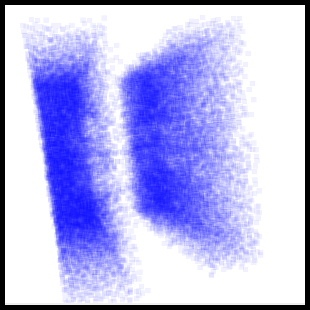
\includegraphics[width=50mm]{waterpoint}
  \end{center}
  \caption{Water point visualisation. Each point represents a water molecule.}
  \label{fig:implementation_waterpoint}
\end{figure}

% }}}

\subsection*{Ball-and-stick}
% {{{

The colour and size of the spheres used to represent the oxygen and hydrogen
atoms are configurable. Similarly, the cylinder size and colour representing
the bonds can be configured. By changing the sphere sizes, the ball-and-stick
visualisation technique can be made to mimic the CPK approach.

Lighting can be enabled to better see the spheres.

Figure \ref{fig:implementation_ballstick} shows some water molecules rendered
using the ball-and-stick visualisation technique. The red spheres represent
oxygen atoms, while the blue spheres represent hydrogen atoms. The
left image uses the classical approach, where cylinders are used to connect the
atoms together. The right image uses the CPK approach, where the atoms are
enlarged to encompass the molecular bond.

\begin{figure}
  \begin{center}
    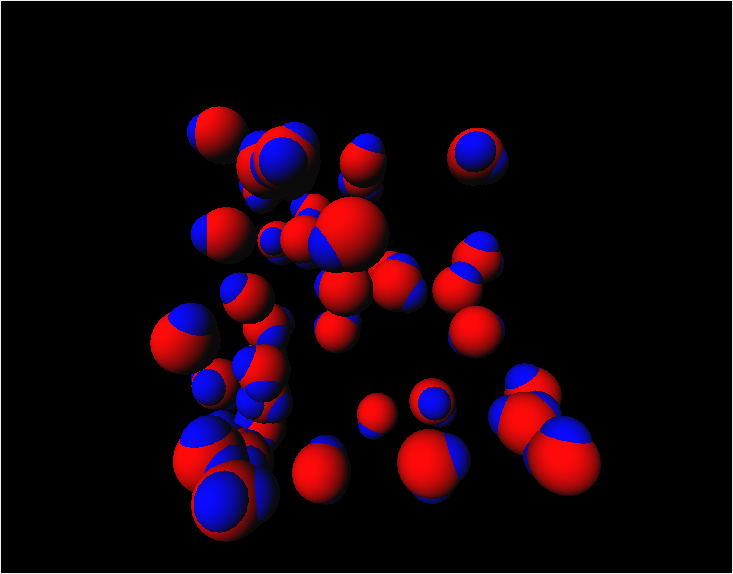
\includegraphics[width=100mm]{ballstick}
  \end{center}
  \caption{Ball-and-stick visualisation. The left image uses the classical
  approach, while the right image uses the CPK approach.}
  \label{fig:implementation_ballstick}
\end{figure}

% }}}

\subsection*{Metaballs}
% {{{

Due to the large number of water molecules, performing a na\"ive comparison
against all the water molecules is very inefficient. Instead, a grid is used to
place the water molecules and test for whether a point is inside or outside a
region of water.

The step size for sampling the volume and the threshold value to use in
determining the surface can all be configured in the user interface. The
threshold value is the main determinant in what the output surface looks like.

% {{{

For the metaballs visualisation technique, a surface needs to be extracted; the
marching cubes and marching tetrahedrons surface extraction algorithms were
both implemented. The algorithms were compared to one another to determine
which algorithm is preferred. The various aspects compared were:

\begin{itemize}

  \item Time for surface extraction - time required to extract the surfaces
  from the volume data.

  \item Surface primitive count - number of surface primitives generated for
  the volume.

  \item Surface quality - the extracted surfaces are visually compared for
  noticeable differences.

\end{itemize}

The two algorithms were tested on the datasets used for the quantisation
experiment (Chapter \ref{cha:experiment}).

Table \ref{tab:appendix_surface_time} in Appendix \ref{cha:tables}, shows the
time required for extracting the surfaces from the volume data. The results
indicate that marching tetrahedrons requires more time to extract the surface,
the extra time required ranges from 50 to 800 milliseconds more. The extra time
required is not considerably large, but the difference is noticeable.

Table \ref{tab:appendix_surface_count} in Appendix \ref{cha:tables}, shows the
number of surface primitives in the extracted surfaces. The surfaces extracted
by marching tetrahedrons are all composed of at least twice as many surface
primitives as that extracted by marching cubes. The extra surface primitives
will increase rendering cost, as well as time required for decimation. This is
the largest factor used in preferring marching cubes over marching
tetrahedrons.

Figure \ref{fig:implementation_compare} shows the surface extracted from
marching cubes on the left, and the surface extracted by marching tetrahedrons
on the right. The view has been zoomed in to more clearly see the surface
differences. The visual differences between the extracted surfaces are minor,
especially when the view is zoomed out to view the entire volume.

\begin{figure}
  \begin{center}
    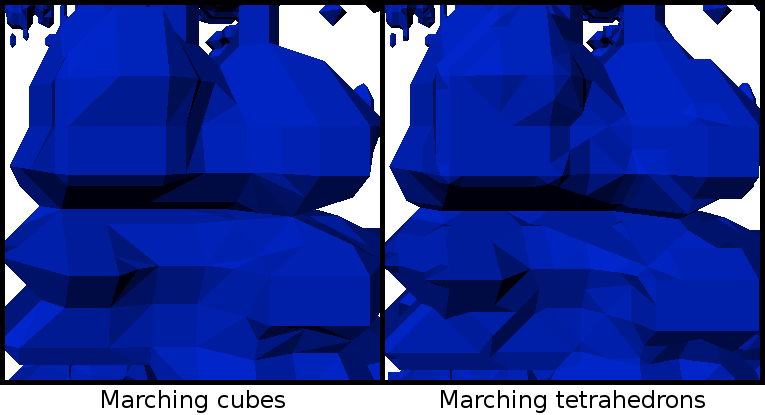
\includegraphics[width=100mm]{surface_compare}
  \end{center}
  \caption{Surface generated by marching cubes (left) and marching tetrahedrons
  (right).}
  \label{fig:implementation_compare}
\end{figure}

As the surface differences are minor, the algorithm that produces fewer
triangles is preferred, which is marching cubes.

% }}}

% {{{

As was mentioned in Section \ref{sec:implementation_details}, the GTS library
is used to perform the surface decimation. Due to unforeseen difficulties and
time constraints, using a library was the fastest way to achieve decimation.

The computational cost for a single frame in the metaballs visualisation is
quite high. A frame can only be generated in real time for small volumes (less
than 500 water molecules). Larger volumes may take upwards of 5 seconds or more
for a single frame to be generated. Performing decimation on the extracted
surface will only increase the computational cost. A pre-processing option is
thus available. All the frames can be pre-processed and saved to file. The
output file is a simple dump of the vertices and normals of all the triangles.
This file can then be used to render the surface without the processing
overhead.

When rendering the surface, one side of the surface is coloured blue, while the
other is coloured green. This allows differentiation of the different sides of
the surface. The blue side of the surface is facing the non-water area of the
volume, while the green side of the surface is facing towards the water area.

Figure \ref{fig:implementation_metaballs} shows the metaballs visualisation for
the data used for Figure \ref{fig:implementation_waterpoint}. The large green
surface on the left part of the figure faces into the left region of water,
behind the surface is a region of non-water. The large blue surface on the
right is the boundary between the region of non-water in the middle, and the
region of water to the right. There are some smaller surfaces in the left and
right areas, which further defines the regions of water.

To help see the surface detail, lighting can be enabled.

\begin{figure}
  \begin{center}
    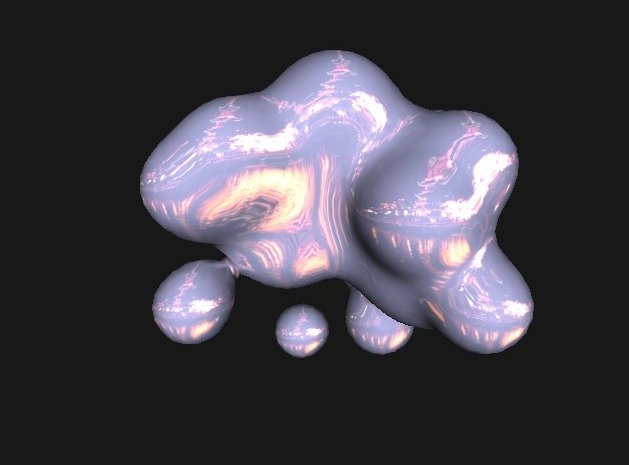
\includegraphics[width=50mm]{metaballs}
  \end{center}
  \caption{Metaballs visualisation. Renders the surface between water and
  non-water molecules.}
  \label{fig:implementation_metaballs}
\end{figure}

% }}}

% }}}

\subsection*{Water cluster}
% {{{

The colour and size of the cylinders used to connect the water molecules
together are all configurable in the user interface.

Lighting can be enabled for this visualisation technique so that the shape and
orientation of the cylinders can be more easily determined.

Figure \ref{fig:implementation_watercluster} shows the water cluster
visualisation where three water clusters are visible. The extracted water
clusters are often quite small, mostly consisting of a few water molecules only.

\begin{figure}
  \begin{center}
    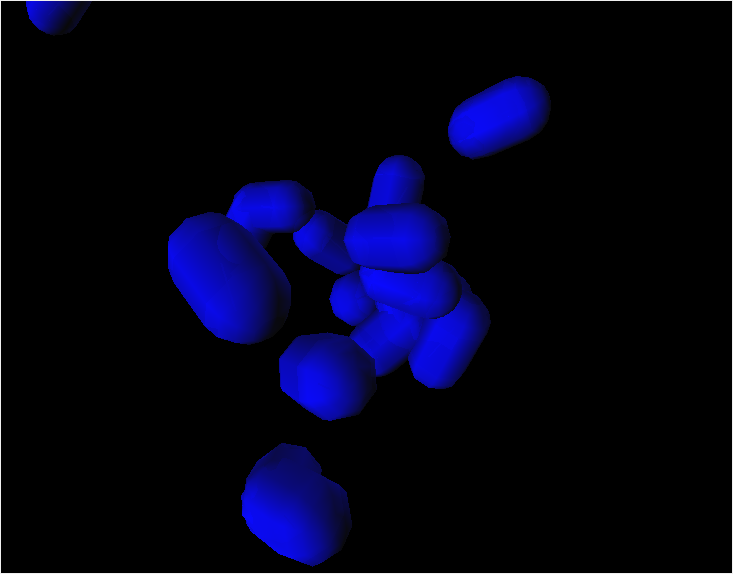
\includegraphics[width=50mm]{watercluster}
  \end{center}
  \caption{Water cluster visualisation. Water molecules within cluster are
  joined using cylinders.}
  \label{fig:implementation_watercluster}
\end{figure}

% }}}

\subsection*{Quantisation error}
% {{{

The starting and final error colours and values are all configurable from
within the user interface.

Figure \ref{fig:implementation_quanterror} shows the quantisation errors for
the example volume used in this chapter. The point rendering (left) and line
rendering (right) modes are shown in the figure. The point rendering renders a
point for the water molecule, while the line rendering renders a line between
the original and quantised positions.

The red areas indicate large quantisation error, while the fainter green areas
indicate lower quantisation error. Due to the stepped colour scale, the
different areas are clearly visible.

\begin{figure}
  \begin{center}
    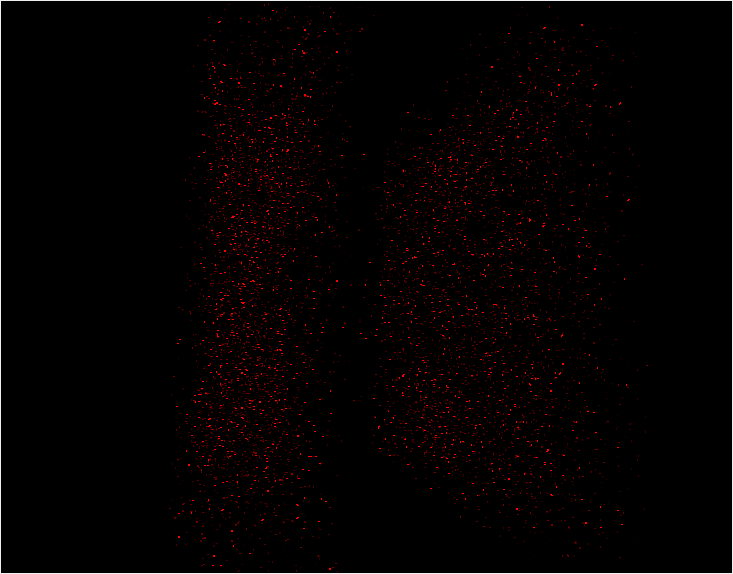
\includegraphics[width=120mm]{quanterror}
  \end{center}
  \caption{Quantisation error visualisation. Quantisation errors are visualised
  using either points (left) or lines (right).}
  \label{fig:implementation_quanterror}
\end{figure}

% }}}

% }}}

\section{Limitations}
% {{{
\label{sec:implementation_limitations}

As the data can be very different, some adjustments to various configuration
values will need to be made to most effectively visualise the data. An example
of such a change is the alpha value and point size for the water point
visualisation technique. For small volumes, a high alpha value and point size
will be needed to effectively visualise the volume. Other changes will need to
be made for the other visualisation techniques. These changes are unfortunately
unavoidable.

The water point visualisation technique is only useful for volumes where there
are large amounts of water and non-water. If the volume is small or uniformly
filled with water molecules, the alpha effects will not be significant.

The metaballs visualisation technique requires considerable processing for each
frame (surface extraction and decimation), hence real time rendering is only
possible for small volumes. The amount of rendering time required is dependant
on the number of water molecules and extracted surface, processing time for a
single frame can be from a few seconds, up to a minute. Disabling decimation
will decrease the time required for a single frame, processing time then ranges
from a few hundred milliseconds, up to 10 seconds.

There is an option to pre-process the volume and save the extracted surfaces to
file, however, the generated files are generally considerably larger than the
DCD file. The size of the pre-processed file is dependant on the number of
water molecules and number of frames. From the data used for the quantisation
experiment, the pre-processed file were an average of 10 times larger than the
DCD file. The smallest output file was the same size as the DCD file, while the
largest was 100 times larger.

To limit the file size and pre-processing time, the number of frames to
pre-process is limited. This number can be set by the user.

% }}}

% }}}

